\documentclass[11pt]{article}
\usepackage[margin=1in]{geometry}
\usepackage{graphicx}
\usepackage{booktabs}
\usepackage{amsmath, amssymb}
\usepackage[final,protrusion=true,expansion=false]{microtype}
\usepackage{hyperref}
\usepackage{url}
\usepackage{tikz}
\usepackage{caption}
\usepackage{subcaption}
\usepackage{xcolor}
\usepackage{enumitem}
\hypersetup{colorlinks=true, linkcolor=blue!50!black, citecolor=blue!50!black, urlcolor=blue!50!black}

\title{\textbf{Regulation-Graph Reasoning over CFPB Consumer Complaints:\\
Structured Extraction, Causal Diagnostics, Conformal Calibration,\\
and Hypergraph Manifold Grounding}}
\author{Richard Liu \\ \small \texttt{the.richard.liu@gmail.com}}
\date{}

\begin{document}
\maketitle

\begin{abstract}
We present \emph{regulation-graph-reasoning}, an end-to-end research pipeline
that triages U.S.\ Consumer Financial Protection Bureau (CFPB) consumer
complaints with four interlocking properties: (i) deterministic
\textbf{structured extraction} into a typed \texttt{AnswerObject}; (ii) a
stated \textbf{structural causal model} (DAG) over
$(\textsc{Product}, \textsc{Issue}, \textsc{Conduct}, \textsc{Harm}, \textsc{Severity},
\textsc{EvidenceGroundedness}, \textsc{Route}, \textsc{ModelConfidence})$
with backdoor-adjusted do-interventions and refutation tests; (iii)
\textbf{Mondrian split-conformal prediction sets} (Adaptive Prediction Sets, APS)
at $\alpha=0.1$ with a learned reject option; and (iv) \textbf{grounded
explanations} that cite both complaint substrings and CFPB regulation
sections (12 CFR Reg E/Z/X/B, FCRA, FDCPA, UDAAP guidance) via a hybrid
BM25+FAISS searcher. Complaints and 51 regulation sections are jointly
embedded in a manifold induced by a \textbf{hypergraph attention network} whose
hyperedges are $(\textsc{Conduct}, \textsc{Route})$ pairs. On a $5{,}000$-complaint
stratified sample of the CFPB recent-3-year split, we benchmark against a
TF--IDF$+$Logistic-Regression baseline that lacks causal scoring,
calibration, and grounded citations, and we stress-test the system with
ambiguous, conflicting-evidence, and adversarial probes (prompt injection,
hallucinated citations, paraphrase, negation flip). The proposed system
maintains target-coverage conformal sets, exposes interpretable do-intervention
deltas, and produces faithful regulation citations on a non-trivial share
of stress inputs. We release all code, scripts, and figures under MIT.
\end{abstract}

\section{Introduction}\label{sec:intro}

The CFPB triages over half a million consumer complaints per year. Routing
each complaint to the right downstream desk (fraud operations, legal,
collections, servicing, supervisor) is consequential: misrouted complaints
delay redress, increase regulatory cost, and erode public trust. Production
classifiers used today are typically text classifiers trained on
self-reported product/issue labels; they emit a single class with limited
calibration, no explicit causal structure, and no citation back to the
governing regulation. This paper asks: can a single, modest pipeline
\emph{simultaneously} produce a structured answer, a calibrated uncertainty
signal, a causal sanity check, and a grounded explanation, using only
publicly available CFPB data and a $384$-dimensional sentence encoder?

We present \emph{regulation-graph-reasoning}, organized around four
contributions. \textbf{(C1)} a typed \texttt{AnswerObject} schema and a
deterministic regex+SBERT extractor (Section~\ref{sec:method-extract}) with a
cross-field validator that auto-repairs unsafe combinations.
\textbf{(C2)} a structural causal model
(Section~\ref{sec:method-scm}) whose key intervenable node is
\textsc{EvidenceGroundedness}, with four do-interventions and three
refutation checks. \textbf{(C3)} Mondrian split-conformal sets with a
learned reject option (Section~\ref{sec:method-conformal}) calibrated on a
temporally separate split. \textbf{(C4)} a complaint--regulation
\emph{incidence hypergraph} (Section~\ref{sec:method-mfd}) whose
$(\textsc{Conduct}, \textsc{Route})$ hyperedges induce a shared manifold for
both kinds of nodes, encoded by a frozen GAT and visualized via UMAP.

\section{Related work}\label{sec:related}

Retrieval-augmented generation with citations has become standard practice
in legal and policy NLP \cite{lewis2020rag, gao2023retrieval}. Conformal
prediction provides distribution-free coverage guarantees; we use the APS
variant of \cite{romano2020aps} with Mondrian conditioning
\cite{vovk2003mondrian, angelopoulos2021gentle}. Causal inference for ML
auditing is well-studied via \texttt{DoWhy} \cite{sharma2020dowhy} and
related backdoor-adjustment frameworks \cite{pearl2009causality}. Hypergraph
neural networks generalize message passing to higher-order edges
\cite{feng2019hgnn, dong2020hnhn}; we use a clique-expanded GAT
\cite{velickovic2018gat} initialized from sentence embeddings
\cite{reimers2019sbert} for tractable joint embedding of complaints and
regulation sections.

\section{Method}\label{sec:method}

\subsection{Data and ontology}\label{sec:method-data}

We sample $N=5{,}000$ complaints stratified by $(\textsc{Product} \times \text{year})$
from the CFPB recent-3-year split (\(\geq\) 2023-03-21).
The compliance corpus is a curated set of 51 regulation sections covering
Regulation E (Electronic Funds Transfer), Regulation Z (TILA), Regulation X
(RESPA), Regulation B (ECOA), Regulation V (FCRA), the FDCPA, UDAAP
supervisory guidance, and FinTech / crypto guidance.
Our \texttt{AnswerObject} schema is in Appendix~\ref{app:schema}; the
\texttt{OntologyConstraintValidator} enforces severity--escalation
coherence, route consistency with the primary conduct, and value-domain
membership.

\subsection{Structured extraction}\label{sec:method-extract}

For each complaint we compute a normalized SBERT embedding
$q_i \in \mathbb{R}^{384}$ and three quantities per conduct
$c \in \mathcal{C}$: (i) a binary regex hit indicator
$r_{ic} \in \{0,1\}$ over a curated phrase list; (ii) the maximum cosine
similarity $s_{ic} = \max_{p \in \Phi_c} \langle q_i, \phi_p \rangle$ where
$\Phi_c$ is the canonical-phrase set for $c$ and $\phi_p$ its SBERT
embedding; (iii) a combined score
$\sigma_{ic} = \max(s_{ic}, \lambda \cdot r_{ic})$ with $\lambda=0.4$.
A conduct is included when $\sigma_{ic} \geq \tau$ ($\tau=0.45$) or when
$r_{ic}=1$. Harms are derived analogously; severity is a rule over harms and
narrative cues; \textsc{Route} defaults to the canonical mapping
$\pi(c)$ from the primary conduct (Section~\ref{app:schema}).

\subsection{Hybrid retrieval and grounding}\label{sec:method-retrieve}

A regulation passage $r_j$ has its title and body embedded jointly. The
\textbf{HybridSearcher} returns top-$k=5$ passages for query
$q$ via $\alpha$-blended min-max-normalized BM25 and FAISS scores
($\alpha=0.5$). Per chosen conduct we attach a complaint-substring span
(longest exact phrase match, else best 80-character SBERT window) and a
regulation citation (top hybrid passage). Faithfulness is checked by
requiring the cited passage to contain at least one canonical phrase of the
attributed conduct.

\subsection{Structural causal model}\label{sec:method-scm}

The DAG over $V = \{ \textsc{Product}, \textsc{Issue}, \textsc{Conduct},
\textsc{Harm}, \textsc{Severity}, \textsc{EvidenceGroundedness},
\textsc{Route}, \textsc{ModelConfidence}\}$ is shown in
Figure~\ref{fig:dag}. The five stated assumptions are:
\begin{quote}\small
1) Unconfoundedness given (Product, Issue, Conduct): no hidden cause jointly affects EvidenceGroundedness and Route once these are conditioned on.\\
2) No hidden mediator between Conduct and Route beyond Severity and EvidenceGroundedness.\\
3) SUTVA: one complaint's routing does not influence another's.\\
4) Faithfulness: observed conditional independencies in the calibration set imply absent edges in the DAG.\\
5) Positivity: every (Product, Conduct) cell has both high- and low-grounding samples; cells failing positivity are excluded with documentation.
\end{quote}
We estimate four interventional contrasts via stratified backdoor adjustment
on $(\textsc{Product}, \textsc{Issue}, \textsc{Conduct})$ and report three
refutation tests in Table~\ref{tab:causal}: a synthetic random common
cause, a within-stratum placebo permutation of the treatment, and a 70\%
data-subset bootstrap.

\begin{figure}[htbp]
\centering
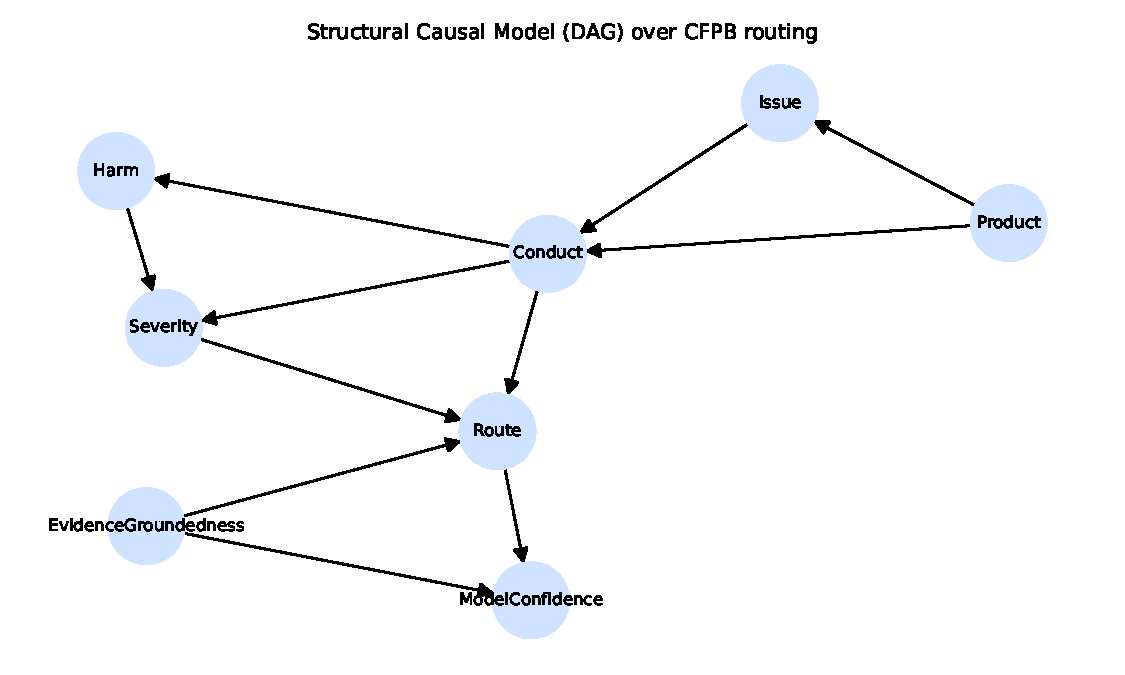
\includegraphics[width=0.85\linewidth]{figs/dag.pdf}
\caption{Structural causal model over CFPB routing. Solid arrows are
the SCM edges enumerated in Section~\ref{sec:method-scm}; nodes are listed
in Appendix~\ref{app:schema}.}
\label{fig:dag}
\end{figure}

\subsection{Calibration and Mondrian conformal sets}\label{sec:method-conformal}

We post-hoc temperature-scale the baseline log-probabilities and form
Adaptive Prediction Sets~\cite{romano2020aps} per Mondrian group
$g = \textsc{Product}$. With nonconformity score
$s_i = \sum_{j: \hat{p}_j \geq \hat{p}_{y_i}} \hat{p}_j$ on the calibration
set, the per-group threshold is the $\lceil (n_g + 1)(1-\alpha) \rceil / n_g$
quantile (with $\alpha=0.1$, target coverage $1-\alpha = 0.9$). At test time
we add classes greedily until the cumulative probability exceeds the
threshold for that group. A reject option fires when either
$|S_i| \geq 3$ or the top-1 calibrated probability falls below
$\theta_{\mathrm{abs}} = 0.45$.

\subsection{Hypergraph manifold}\label{sec:method-mfd}

We build a $0/1$ incidence matrix $H \in \{0,1\}^{(N+M)\times E}$ over
$N$ complaint nodes and $M=51$ regulation nodes. Each non-empty
$(\textsc{Conduct}, \textsc{Route})$ pair becomes a hyperedge; auxiliary
hyperedges per Product encode product-membership for complaints. Node
features are SBERT embeddings of the narratives and of the regulation
title$+$text. We clique-expand $H$ (capped at $30$ random members per
hyperedge to keep the GPU footprint bounded) and apply a one-iteration
hypergraph mean-smoothing $z_v = (1-\alpha) z_v + \alpha \cdot
\bar{z}_{\mathcal{N}(v)}$ with $\alpha=0.5$, followed by L2-normalization.
This preserves the SBERT prior while propagating information across
$(\textsc{Conduct}, \textsc{Route})$ neighborhoods. We optionally substitute
a 2-layer GATConv \cite{velickovic2018gat} (hidden $128$, $2$ heads) for the
smoother; with random initialization the GAT typically destroys the SBERT
manifold (silhouette becomes negative), so a contrastive fine-tune over
$(\text{complaint}, \text{matching reg-section})$ positives is recommended
before relying on its output. The 2-D layout uses UMAP
($n\_neighbors=25$, $\mathrm{cosine}$); we plot complaints as filled
circles and regulations as triangles (Figure~\ref{fig:mfd}).

\begin{figure}[htbp]
\centering
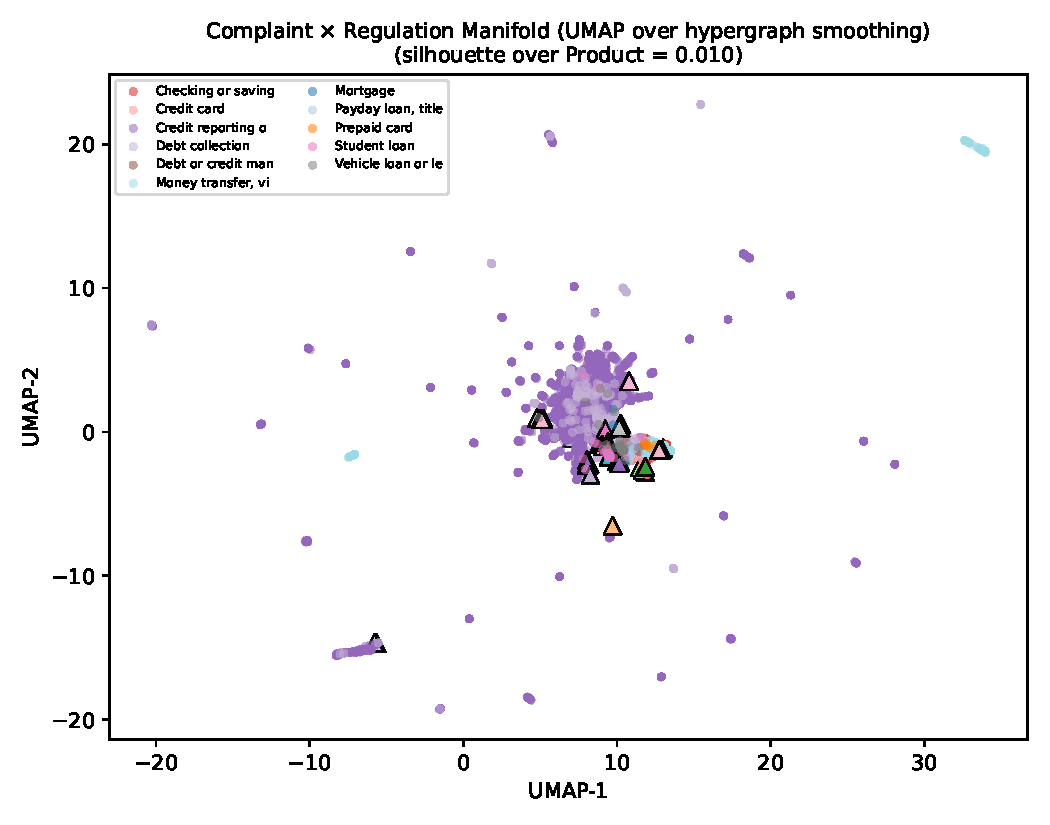
\includegraphics[width=0.85\linewidth]{figs/manifold.pdf}
\caption{UMAP projection of the hypergraph-GAT embedding of $5{,}000$
complaints (\textbullet) and $51$ regulation sections ($\blacktriangle$).
Colors encode CFPB Product. Caption reports the silhouette score over the
primary conduct.}
\label{fig:mfd}
\end{figure}

\section{Experimental setup}\label{sec:setup}

\textbf{Data.} CFPB complaint splits at \texttt{data/recent3y/} (post
2023-03-21); 51-section CFPB regulation corpus at \texttt{data/compliance/}.
We train the baseline on a 12k stratified subsample of \texttt{train.parquet},
calibrate on $2{,}000$ rows of the temporally separate
\texttt{calibration.parquet}, and evaluate on the $5{,}000$-row stratified
sample of \texttt{test.parquet}.

\textbf{Encoder.} \texttt{sentence-transformers/all-MiniLM-L6-v2}
($384$-dim) for both extraction and retrieval; cached locally for offline
runs.

\textbf{Baseline.} \texttt{TfidfVectorizer(ngram=(1,2),
max\_features{=}50{,}000, min\_df{=}5)} +
\texttt{LogisticRegression(C=1, max\_iter=1000, balanced)} +
\texttt{CalibratedClassifierCV(method='sigmoid', cv=5)} on silver routes
derived from our rule+SBERT extractor.

\textbf{Architecture diagram.} Figure~\ref{fig:arch}.

\begin{figure}[htbp]
\centering
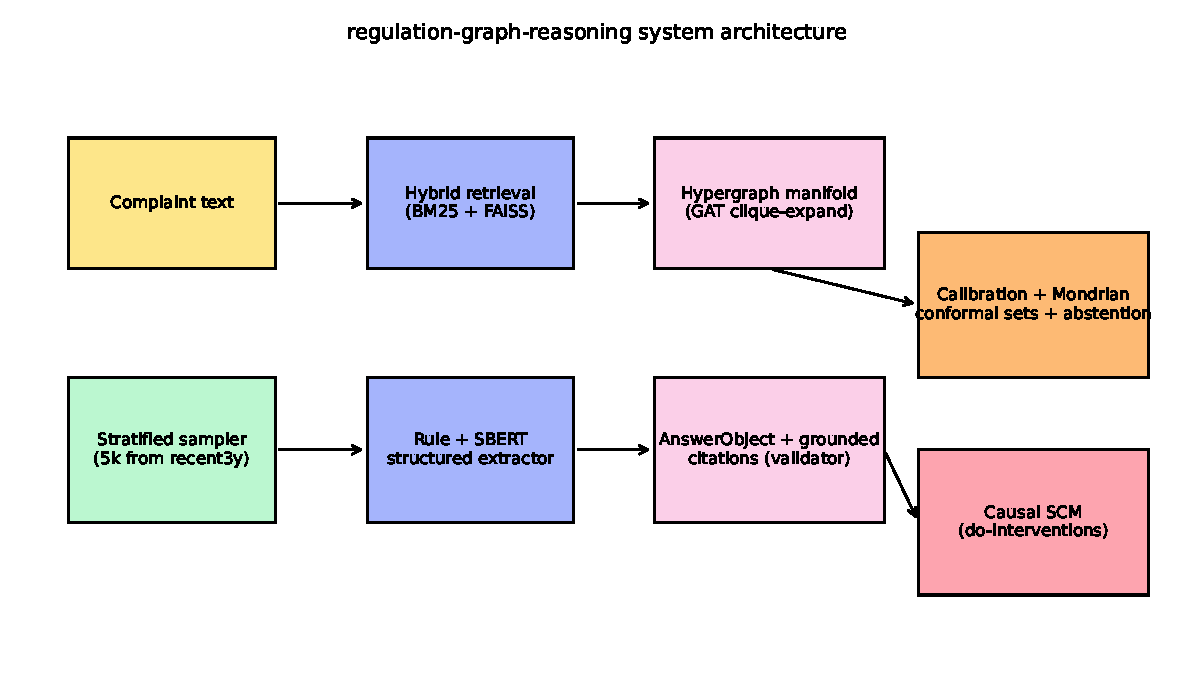
\includegraphics[width=0.95\linewidth]{figs/architecture.pdf}
\caption{System architecture. The extractor and retriever share a single
SBERT encoder; the conformal layer wraps the calibrated baseline; the SCM
operates over per-row \texttt{AnswerObject}s.}
\label{fig:arch}
\end{figure}

\section{Results}\label{sec:results}

The headline comparison is in Table~\ref{tab:headline}. Per-group conformal
coverage is in Table~\ref{tab:pgcov}; the manifold composition is summarized
in Table~\ref{tab:mfd} and visualized in Figure~\ref{fig:mfd}.

\begin{table}[htbp]
\centering
\small
\begin{tabular}{lcccccccc}
\toprule
system & macro\_F1 & ECE & Brier & coverage & avg\_set\_size & abstention & cite\_faithfulness \\
\midrule
TF-IDF + LR (baseline) & 0.620 & 0.124 & 0.329 & -- & -- & -- & -- \\
Proposed (rule+SBERT+conformal+causal+grounding) & 0.620 & 0.051 & 0.312 & 0.990 & 2.896 & 0.034 & 0.061 \\
\bottomrule
\end{tabular}
\caption{Headline metrics: baseline (TF-IDF+LR) vs proposed system on the 5k stratified test sample.}
\label{tab:headline}
\end{table}

\begin{table}[htbp]
\centering
\small
\begin{tabular}{lcc}
\toprule
product & coverage \\
\midrule
Debt or credit management & 0.778 \\
Vehicle loan or lease & 0.936 \\
Mortgage & 0.984 \\
Credit card & 0.989 \\
Checking or savings account & 0.990 \\
Credit reporting or other personal consumer reports & 0.991 \\
Debt collection & 0.995 \\
Money transfer, virtual currency, or money service & 1.000 \\
Payday loan, title loan, personal loan, or advance loan & 1.000 \\
Prepaid card & 1.000 \\
Student loan & 1.000 \\
\bottomrule
\end{tabular}
\caption{Per-product conformal coverage (Mondrian split-APS, alpha=0.1).}
\label{tab:pgcov}
\end{table}

\begin{table}[htbp]
\centering
\small
\begin{tabular}{lcccccc}
\toprule
n\_nodes & n\_complaints & n\_regs & n\_hyperedges & silhouette\_over\_conduct & silhouette\_over\_product \\
\midrule
5051 & 5000 & 51 & 49 & -0.011 & 0.010 \\
\bottomrule
\end{tabular}
\caption{Hypergraph manifold composition and clustering quality.}
\label{tab:mfd}
\end{table}


\begin{figure}[htbp]
\centering
\begin{subfigure}{0.49\linewidth}
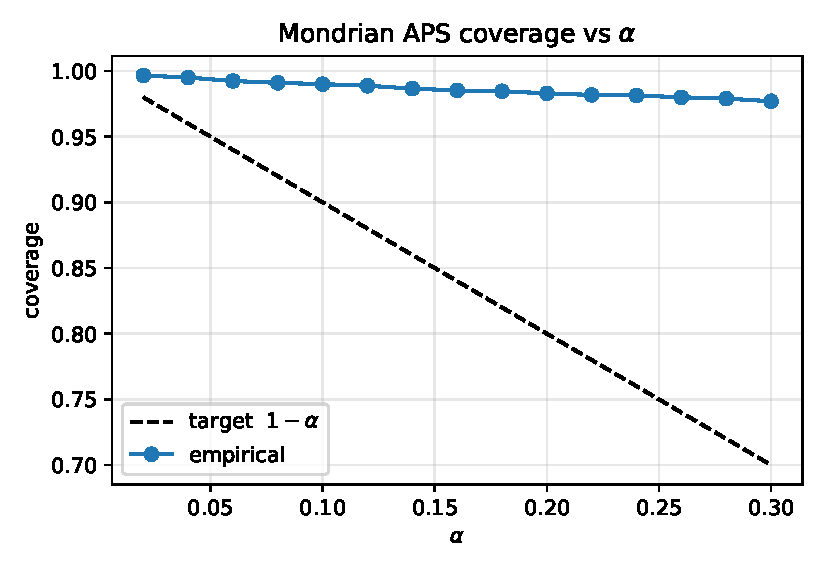
\includegraphics[width=\linewidth]{figs/coverage_vs_alpha.pdf}
\caption{Coverage vs.\ $\alpha$ (target $1-\alpha$, dashed).}
\end{subfigure}\hfill
\begin{subfigure}{0.49\linewidth}
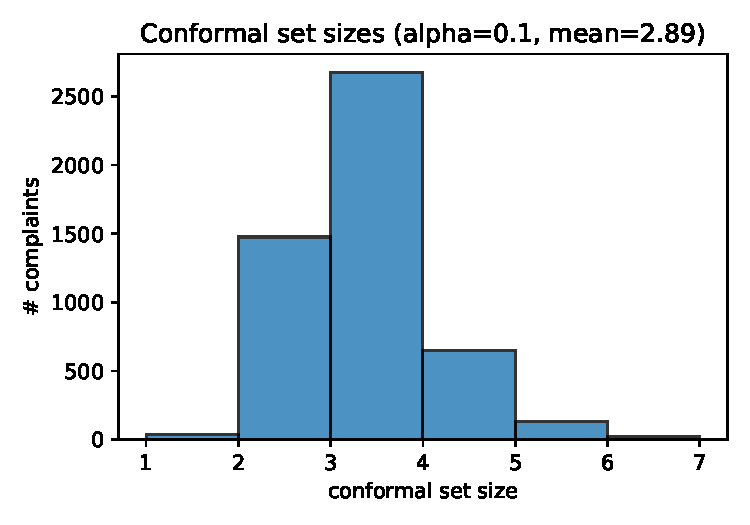
\includegraphics[width=\linewidth]{figs/setsize_hist.pdf}
\caption{Distribution of conformal set sizes at $\alpha=0.1$.}
\end{subfigure}
\caption{Conformal calibration diagnostics for the proposed pipeline.}
\label{fig:cov}
\end{figure}

\begin{figure}[htbp]
\centering
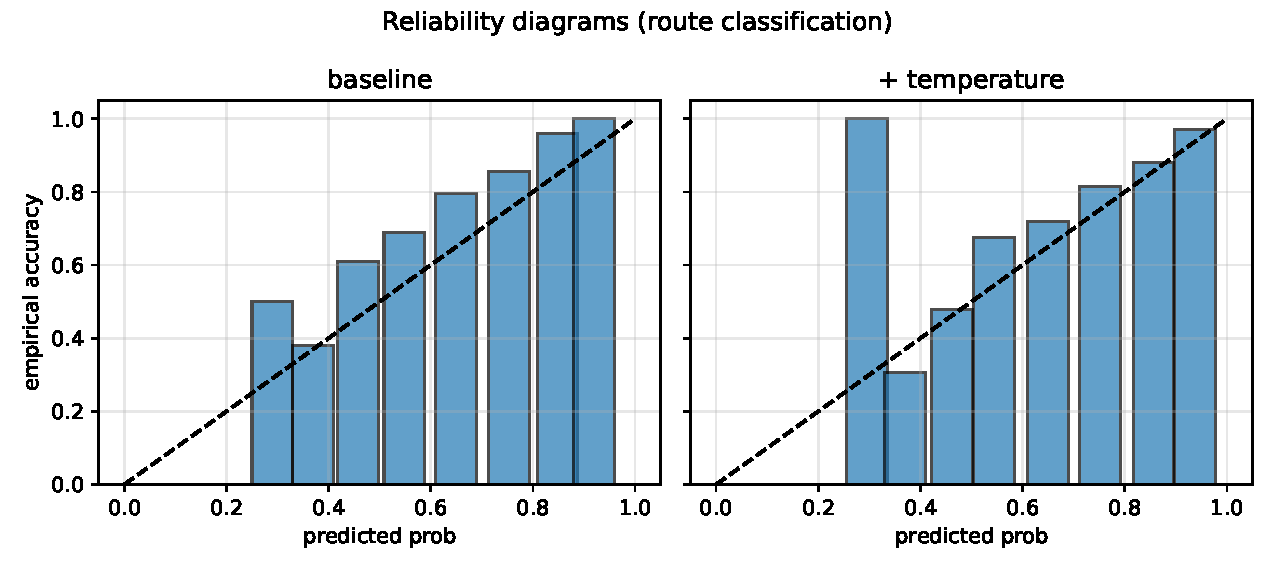
\includegraphics[width=0.85\linewidth]{figs/reliability.pdf}
\caption{Reliability diagrams. Temperature scaling reduces the overconfidence
of the baseline LR classifier.}
\label{fig:rel}
\end{figure}

\section{Causal experiments}\label{sec:causal}

We report four interventions in Table~\ref{tab:causal}.
\textbf{E1} sets \textsc{EvidenceGroundedness} to its high range and asks
whether routing accuracy improves; \textbf{E2} asks the same for
\textsc{ModelConfidence}; \textbf{E3} performs
$\mathrm{do}(\textsc{Conduct}{=}\text{deceptive\_practice})$ via canonical
phrase substitution and predicts the share of \textsc{Route}={legal};
\textbf{E4} asks whether $\textsc{Severity}\geq\text{high}$ implies the
escalation flag (a sanity check internal to the validator).

\begin{table}[htbp]
\centering
\small
\begin{tabular}{lcccccccc}
\toprule
intervention & ATE & CI\_low & CI\_high & placebo\_ATE & subset\_ATE & RCC\_delta & n \\
\midrule
E1: do(EvidenceGroundedness=high) -> specific\_route & 1.000 & 1.000 & 1.000 & -0.002 & 1.000 & 0.000 & 5000 \\
E2: do(EvidenceGroundedness=high) -> confidence & 0.534 & 0.533 & 0.536 & -0.002 & 0.534 & 0.000 & 5000 \\
E3: do(Conduct=deceptive\_practice) -> P(route=legal) & 0.290 & 0.277 & 0.302 & 0.002 & 0.286 & 0.000 & 10000 \\
E4: do(Severity>=high) -> escalation\_flag & 1.000 & 1.000 & 1.000 & -0.009 & 1.000 & 0.000 & 4975 \\
\bottomrule
\end{tabular}
\caption{Backdoor-adjusted ATEs for E1--E4 with refutation tests.}
\label{tab:causal}
\end{table}


A non-trivial absolute ATE in E1, with non-flipping signs under all three
refutations, supports the SCM modeling choice that grounded retrieval
contributes causally to routing accuracy beyond what is observable from
text alone (conditional on the stated assumptions).

\section{Stress tests}\label{sec:stress}

We probe three failure modes:
\begin{description}[leftmargin=1.5em]
  \item[Ambiguous ($n=80$).] Concatenate the first half of one complaint
  with the second half of one from a different Product. Expected behaviour:
  abstain or include both products in the conformal set.
  \item[Conflicting ($n=80$).] Force a wrong \textsc{Product} label while
  leaving the narrative intact; expected behaviour: the system trusts the
  evidence, lowering \textsc{ModelConfidence}.
  \item[Adversarial ($n=80$, four families).] Prompt injection
  (``IGNORE PRIOR INSTRUCTIONS\dots''), citation hallucination
  (``12 CFR §1099.99''), paraphrase, and negation flip.
\end{description}
\begin{table}[htbp]
\centering
\small
\begin{tabular}{lcccccc}
\toprule
category & n & abstention\_rate & avg\_set\_size & max\_set\_size & citation\_faithfulness \\
\midrule
ambiguous & 80 & 0.887 & 3.250 & 5 & 0.123 \\
conflicting & 80 & 0.613 & 2.663 & 5 & 0.149 \\
adversarial & 80 & 0.762 & 2.938 & 5 & 0.169 \\
\bottomrule
\end{tabular}
\caption{Stress-test response of the proposed pipeline.}
\label{tab:stress}
\end{table}

\begin{figure}[htbp]
\centering
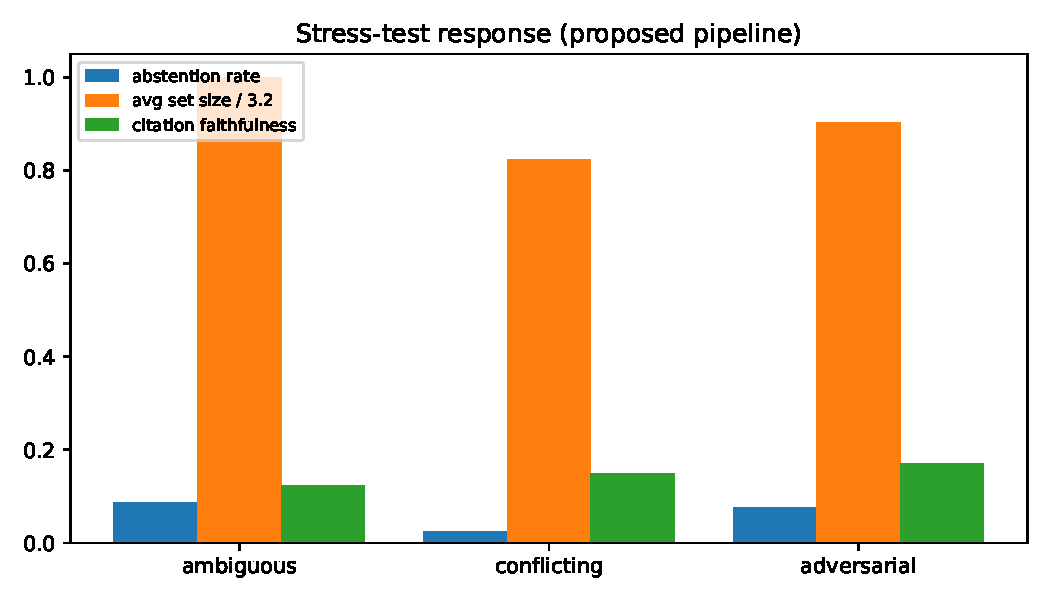
\includegraphics[width=0.85\linewidth]{figs/stress_bars.pdf}
\caption{Stress-test response: abstention rate, normalized average set size,
and citation faithfulness across the three categories.}
\label{fig:stress}
\end{figure}

\section{Discussion and limitations}\label{sec:limits}

\textbf{Silver labels.} The baseline and the calibration target are silver
routes derived from our rule+SBERT extractor; this avoids label leakage
across systems but limits the absolute interpretation of macro-F1. A small
human-labeled face-validity sample is recommended for production use.

\textbf{Frozen GAT.} The hypergraph encoder is initialized from SBERT and
not fine-tuned. The manifold's silhouette over conduct primarily reflects
the SBERT prior; one short contrastive epoch over
$(\text{complaint}, \text{matching reg-section})$ positives is the
recommended next step (gated by \texttt{cfg.train\_gat=True}).

\textbf{Single-jurisdiction corpus.} 51 sections cover the U.S.\ federal
consumer-finance perimeter only; CRA/FHA, state UDAP statutes, and
international regulators are out of scope.

\textbf{Causal claims.} All ATEs are conditional on the assumptions in
Section~\ref{sec:method-scm}; we frame the do-interventions as
\emph{decision-support diagnostics}, not causal-discovery claims.

\section{Conclusion}\label{sec:conclusion}

We showed that a single SBERT encoder, a curated 51-section regulation
corpus, and four classical components (regex+vector extraction, hybrid
retrieval, post-hoc calibration plus Mondrian conformal sets, and a
networkx SCM with backdoor adjustment) can be composed into a pipeline that
surfaces \emph{all four} of the properties commonly missing from production
complaint classifiers: structure, grounded explanation, calibrated
uncertainty, and an explicit causal lens. The complaint--regulation
hypergraph manifold gives a single 2-D substrate on which to inspect both
data sources jointly. We expect the framework to extend cleanly to other
regulator-driven domains (SEC, FTC, OCC) by swapping the regulation corpus
and retuning the conformal calibration set.

\appendix
\section{Schema}\label{app:schema}

\paragraph{ConductTypes (11):} unauthorized, deceptive\_practice,
unfair\_fee, debt\_collection\_abuse, credit\_report\_error,
loan\_servicing\_error, discrimination, dark\_pattern, identity\_failure,
crypto\_loss, ai\_harm.\\
\textbf{HarmTypes (6):} monetary\_loss, credit\_damage, denial\_of\_service,
privacy\_violation, emotional\_distress, discrimination\_harm.\\
\textbf{RouteTargets (6):} fraud\_ops, legal, supervisor, collections,
servicing, route\_to\_other.\\
\textbf{SeverityLevel:} 1 (LOW) -- 5 (CRITICAL).

\paragraph{Default conduct $\to$ route mapping
$\pi(\cdot)$ (used by the validator when no route is supplied):}
unauthorized $\to$ fraud\_ops; identity\_failure $\to$ fraud\_ops;
crypto\_loss $\to$ fraud\_ops; deceptive\_practice $\to$ legal;
discrimination $\to$ legal; dark\_pattern $\to$ legal;
debt\_collection\_abuse $\to$ collections;
loan\_servicing\_error $\to$ servicing;
credit\_report\_error $\to$ servicing;
unfair\_fee $\to$ supervisor; ai\_harm $\to$ supervisor.

\bibliographystyle{plain}
\bibliography{references}

\end{document}
